% Options for packages loaded elsewhere
\PassOptionsToPackage{unicode}{hyperref}
\PassOptionsToPackage{hyphens}{url}
%
\documentclass[
  9pt,
  ignorenonframetext,
]{beamer}
\usepackage{pgfpages}
\setbeamertemplate{caption}[numbered]
\setbeamertemplate{caption label separator}{: }
\setbeamercolor{caption name}{fg=normal text.fg}
\beamertemplatenavigationsymbolsempty
% Prevent slide breaks in the middle of a paragraph
\widowpenalties 1 10000
\raggedbottom
\setbeamertemplate{part page}{
  \centering
  \begin{beamercolorbox}[sep=16pt,center]{part title}
    \usebeamerfont{part title}\insertpart\par
  \end{beamercolorbox}
}
\setbeamertemplate{section page}{
  \centering
  \begin{beamercolorbox}[sep=12pt,center]{part title}
    \usebeamerfont{section title}\insertsection\par
  \end{beamercolorbox}
}
\setbeamertemplate{subsection page}{
  \centering
  \begin{beamercolorbox}[sep=8pt,center]{part title}
    \usebeamerfont{subsection title}\insertsubsection\par
  \end{beamercolorbox}
}
\AtBeginPart{
  \frame{\partpage}
}
\AtBeginSection{
  \ifbibliography
  \else
    \frame{\sectionpage}
  \fi
}
\AtBeginSubsection{
  \frame{\subsectionpage}
}
\usepackage{lmodern}
\usepackage{amssymb,amsmath}
\usepackage{ifxetex,ifluatex}
\ifnum 0\ifxetex 1\fi\ifluatex 1\fi=0 % if pdftex
  \usepackage[T1]{fontenc}
  \usepackage[utf8]{inputenc}
  \usepackage{textcomp} % provide euro and other symbols
\else % if luatex or xetex
  \usepackage{unicode-math}
  \defaultfontfeatures{Scale=MatchLowercase}
  \defaultfontfeatures[\rmfamily]{Ligatures=TeX,Scale=1}
\fi
\usetheme[]{Berkeley}
\usecolortheme{dove}
\usefonttheme{structurebold}
% Use upquote if available, for straight quotes in verbatim environments
\IfFileExists{upquote.sty}{\usepackage{upquote}}{}
\IfFileExists{microtype.sty}{% use microtype if available
  \usepackage[]{microtype}
  \UseMicrotypeSet[protrusion]{basicmath} % disable protrusion for tt fonts
}{}
\makeatletter
\@ifundefined{KOMAClassName}{% if non-KOMA class
  \IfFileExists{parskip.sty}{%
    \usepackage{parskip}
  }{% else
    \setlength{\parindent}{0pt}
    \setlength{\parskip}{6pt plus 2pt minus 1pt}}
}{% if KOMA class
  \KOMAoptions{parskip=half}}
\makeatother
\usepackage{xcolor}
\IfFileExists{xurl.sty}{\usepackage{xurl}}{} % add URL line breaks if available
\IfFileExists{bookmark.sty}{\usepackage{bookmark}}{\usepackage{hyperref}}
\hypersetup{
  pdftitle={RMarkdown},
  pdfauthor={Frederico Bertholini},
  hidelinks,
  pdfcreator={LaTeX via pandoc}}
\urlstyle{same} % disable monospaced font for URLs
\newif\ifbibliography
\usepackage{color}
\usepackage{fancyvrb}
\newcommand{\VerbBar}{|}
\newcommand{\VERB}{\Verb[commandchars=\\\{\}]}
\DefineVerbatimEnvironment{Highlighting}{Verbatim}{commandchars=\\\{\}}
% Add ',fontsize=\small' for more characters per line
\usepackage{framed}
\definecolor{shadecolor}{RGB}{248,248,248}
\newenvironment{Shaded}{\begin{snugshade}}{\end{snugshade}}
\newcommand{\AlertTok}[1]{\textcolor[rgb]{0.94,0.16,0.16}{#1}}
\newcommand{\AnnotationTok}[1]{\textcolor[rgb]{0.56,0.35,0.01}{\textbf{\textit{#1}}}}
\newcommand{\AttributeTok}[1]{\textcolor[rgb]{0.77,0.63,0.00}{#1}}
\newcommand{\BaseNTok}[1]{\textcolor[rgb]{0.00,0.00,0.81}{#1}}
\newcommand{\BuiltInTok}[1]{#1}
\newcommand{\CharTok}[1]{\textcolor[rgb]{0.31,0.60,0.02}{#1}}
\newcommand{\CommentTok}[1]{\textcolor[rgb]{0.56,0.35,0.01}{\textit{#1}}}
\newcommand{\CommentVarTok}[1]{\textcolor[rgb]{0.56,0.35,0.01}{\textbf{\textit{#1}}}}
\newcommand{\ConstantTok}[1]{\textcolor[rgb]{0.00,0.00,0.00}{#1}}
\newcommand{\ControlFlowTok}[1]{\textcolor[rgb]{0.13,0.29,0.53}{\textbf{#1}}}
\newcommand{\DataTypeTok}[1]{\textcolor[rgb]{0.13,0.29,0.53}{#1}}
\newcommand{\DecValTok}[1]{\textcolor[rgb]{0.00,0.00,0.81}{#1}}
\newcommand{\DocumentationTok}[1]{\textcolor[rgb]{0.56,0.35,0.01}{\textbf{\textit{#1}}}}
\newcommand{\ErrorTok}[1]{\textcolor[rgb]{0.64,0.00,0.00}{\textbf{#1}}}
\newcommand{\ExtensionTok}[1]{#1}
\newcommand{\FloatTok}[1]{\textcolor[rgb]{0.00,0.00,0.81}{#1}}
\newcommand{\FunctionTok}[1]{\textcolor[rgb]{0.00,0.00,0.00}{#1}}
\newcommand{\ImportTok}[1]{#1}
\newcommand{\InformationTok}[1]{\textcolor[rgb]{0.56,0.35,0.01}{\textbf{\textit{#1}}}}
\newcommand{\KeywordTok}[1]{\textcolor[rgb]{0.13,0.29,0.53}{\textbf{#1}}}
\newcommand{\NormalTok}[1]{#1}
\newcommand{\OperatorTok}[1]{\textcolor[rgb]{0.81,0.36,0.00}{\textbf{#1}}}
\newcommand{\OtherTok}[1]{\textcolor[rgb]{0.56,0.35,0.01}{#1}}
\newcommand{\PreprocessorTok}[1]{\textcolor[rgb]{0.56,0.35,0.01}{\textit{#1}}}
\newcommand{\RegionMarkerTok}[1]{#1}
\newcommand{\SpecialCharTok}[1]{\textcolor[rgb]{0.00,0.00,0.00}{#1}}
\newcommand{\SpecialStringTok}[1]{\textcolor[rgb]{0.31,0.60,0.02}{#1}}
\newcommand{\StringTok}[1]{\textcolor[rgb]{0.31,0.60,0.02}{#1}}
\newcommand{\VariableTok}[1]{\textcolor[rgb]{0.00,0.00,0.00}{#1}}
\newcommand{\VerbatimStringTok}[1]{\textcolor[rgb]{0.31,0.60,0.02}{#1}}
\newcommand{\WarningTok}[1]{\textcolor[rgb]{0.56,0.35,0.01}{\textbf{\textit{#1}}}}
\usepackage{graphicx}
\makeatletter
\def\maxwidth{\ifdim\Gin@nat@width>\linewidth\linewidth\else\Gin@nat@width\fi}
\def\maxheight{\ifdim\Gin@nat@height>\textheight\textheight\else\Gin@nat@height\fi}
\makeatother
% Scale images if necessary, so that they will not overflow the page
% margins by default, and it is still possible to overwrite the defaults
% using explicit options in \includegraphics[width, height, ...]{}
\setkeys{Gin}{width=\maxwidth,height=\maxheight,keepaspectratio}
% Set default figure placement to htbp
\makeatletter
\def\fps@figure{htbp}
\makeatother
\setlength{\emergencystretch}{3em} % prevent overfull lines
\providecommand{\tightlist}{%
  \setlength{\itemsep}{0pt}\setlength{\parskip}{0pt}}
\setcounter{secnumdepth}{5}

\title{RMarkdown}
\subtitle{Métodos Quantitativos Aplicados à Ciência Política}
\author{Frederico Bertholini}
\date{09.nov.2020}

\begin{document}
\frame{\titlepage}

\begin{frame}[allowframebreaks]
  \tableofcontents[hideallsubsections]
\end{frame}
\begin{frame}[fragile]{Rode seus pacotes!}
\protect\hypertarget{rode-seus-pacotes}{}
\begin{Shaded}
\begin{Highlighting}[]
\KeywordTok{lapply}\NormalTok{(}\KeywordTok{c}\NormalTok{(}\StringTok{"tidyverse"}\NormalTok{,}\StringTok{"haven"}\NormalTok{,}\StringTok{"lubridate"}\NormalTok{,}
         \StringTok{"janitor"}\NormalTok{,}\StringTok{"readxl"}\NormalTok{,}
          \StringTok{"stringr"}\NormalTok{, }\StringTok{"magrittr"}\NormalTok{,}\StringTok{"srvyr"}\NormalTok{,}
         \StringTok{"survey"}\NormalTok{),require,}\DataTypeTok{character.only=}\NormalTok{T)}
\end{Highlighting}
\end{Shaded}
\end{frame}

\hypertarget{revendo-conteuxfados-da-uxfaltima-aula---gruxe1ficos}{%
\section{Revendo conteúdos da última aula -
gráficos}\label{revendo-conteuxfados-da-uxfaltima-aula---gruxe1ficos}}

\begin{frame}{Refazendo um gráfico feio}
\protect\hypertarget{refazendo-um-gruxe1fico-feio}{}
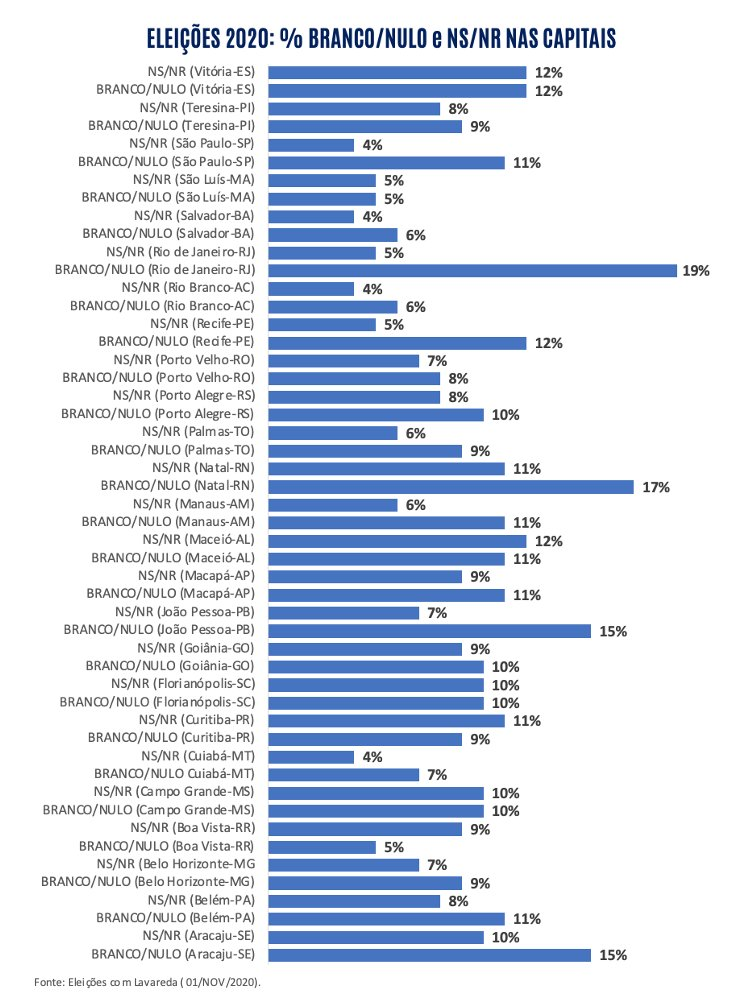
\includegraphics{imgs/grafico_feio.jpeg}
\end{frame}

\begin{frame}{Ficou feio mesmo}
\protect\hypertarget{ficou-feio-mesmo}{}

\includegraphics{imgs/feio_mesmo.png}
\end{frame}

\begin{frame}[fragile]{Então bora melhorar}
\protect\hypertarget{entuxe3o-bora-melhorar}{}
LIVE CODING

\begin{Shaded}
\begin{Highlighting}[]
\KeywordTok{source}\NormalTok{(}\StringTok{"dados/brincando\_graficos.R"}\NormalTok{)}
\end{Highlighting}
\end{Shaded}
\end{frame}

\begin{frame}{}
\protect\hypertarget{section}{}
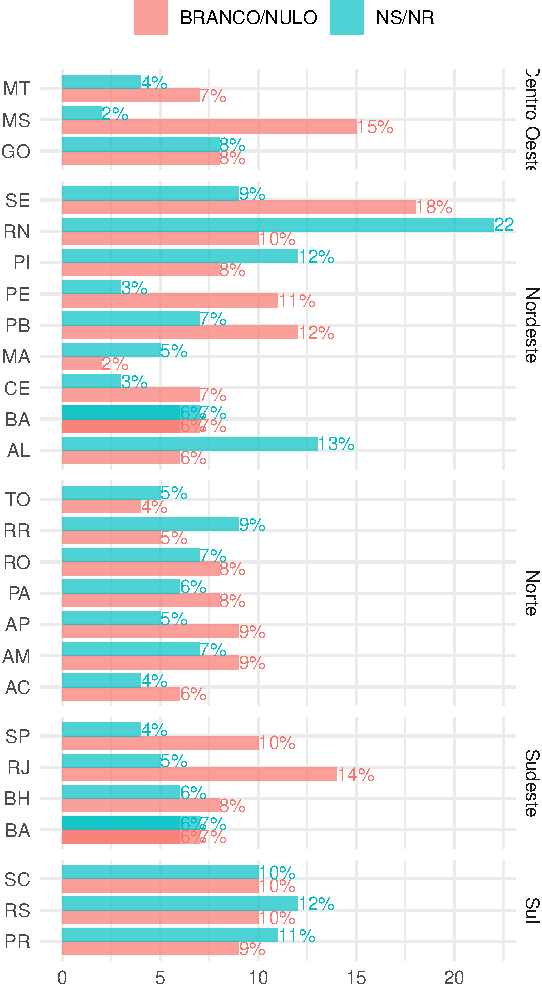
\includegraphics{aula_07_files/figure-beamer/unnamed-chunk-3-1.pdf}
\end{frame}

\begin{frame}{onde estamos?}
\protect\hypertarget{onde-estamos}{}
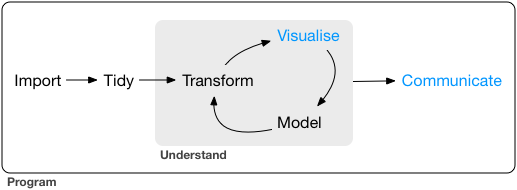
\includegraphics{imgs/data-science-communicate.png}
\end{frame}

\hypertarget{rmarkdown}{%
\section{RMarkdown}\label{rmarkdown}}

\begin{frame}{O que é?}
\protect\hypertarget{o-que-uxe9}{}
\begin{itemize}
\item
  Comunicar com os tomadores de decisão,

  -- que querem se concentrar nas conclusões, não no código por trás da
  análise.
\item
  Colaborar com outros cientistas de dados,

  -- interessados em suas conclusões e como você as alcançou (ou seja, o
  código).
\item
  um caderno de laboratório moderno,

  -- onde você pode anotar não apenas o que fez, mas também o que
  pretende.
\end{itemize}

O R Markdown integra vários pacotes R e ferramentas externas. então, use
o cheatsheets:

\href{https://github.com/rstudio/cheatsheets/raw/master/rmarkdown-2.0.pdf}{R
Markdown Cheat Sheet}

\href{https://www.rstudio.com/wp-content/uploads/2015/03/rmarkdown-reference.pdf}{R
Markdown Reference Guide}
\end{frame}

\begin{frame}{}
\protect\hypertarget{section-1}{}
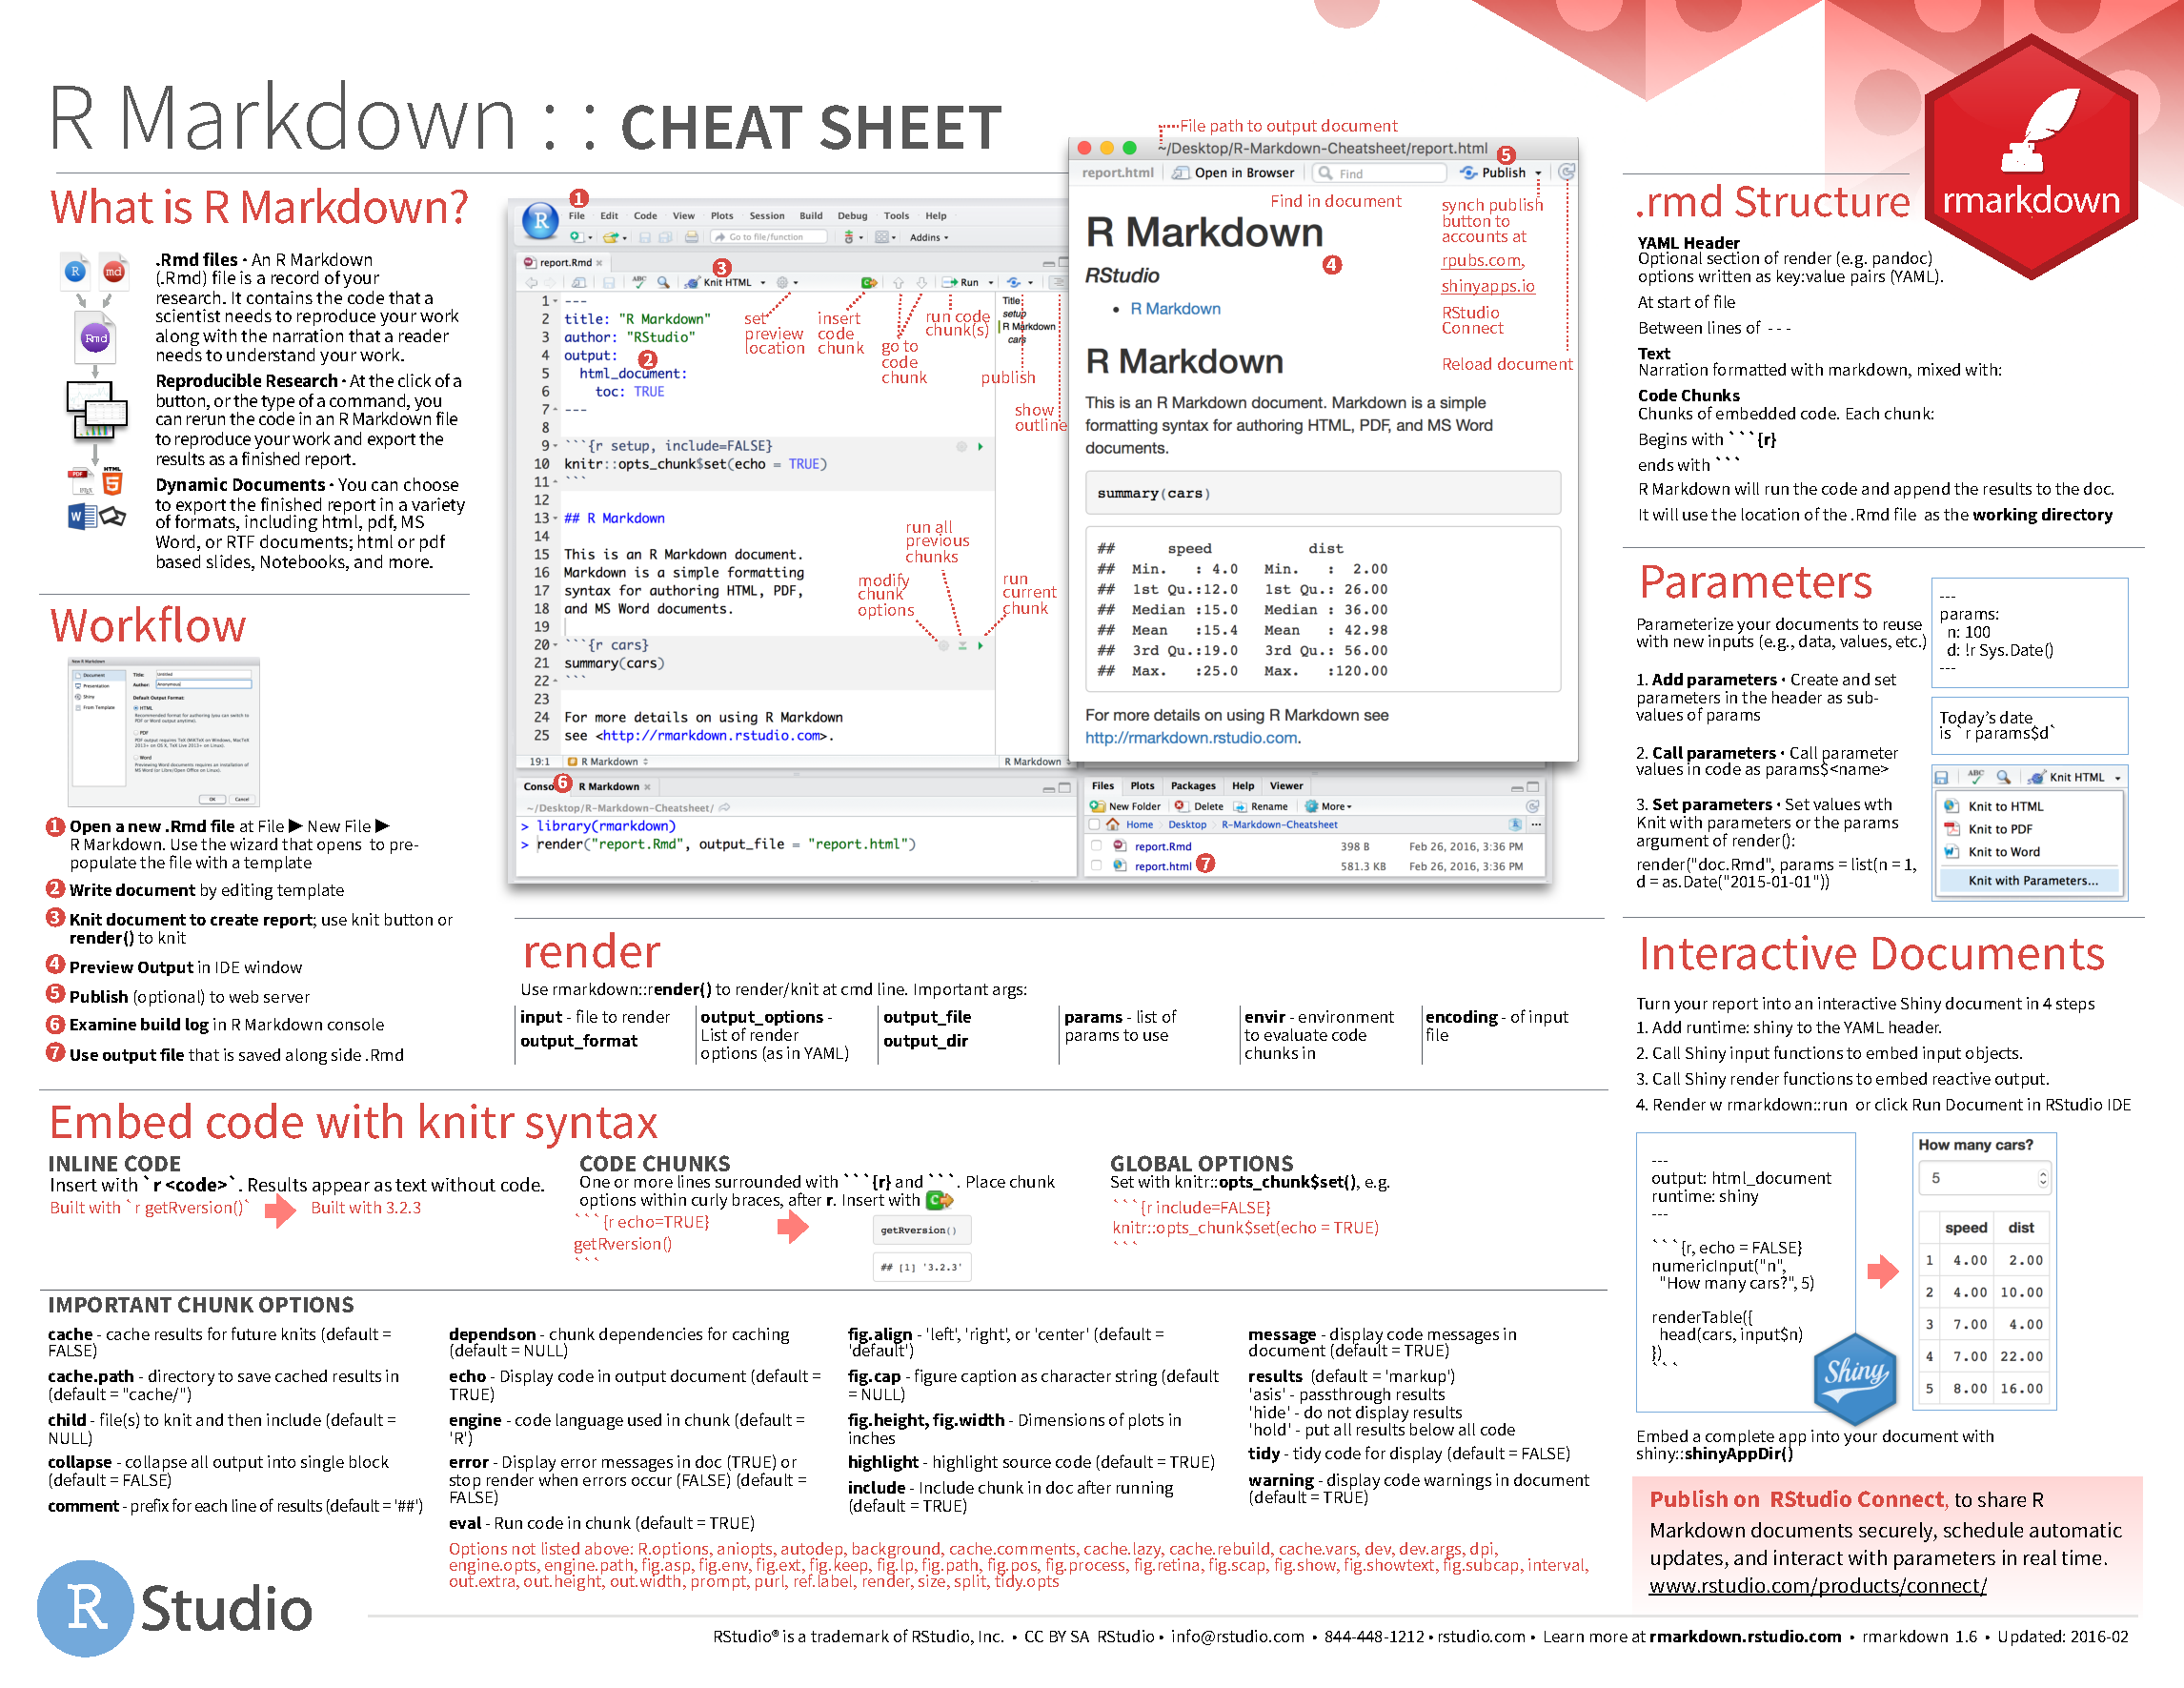
\includegraphics{imgs/rmarkdown}
\end{frame}

\begin{frame}{}
\protect\hypertarget{section-2}{}
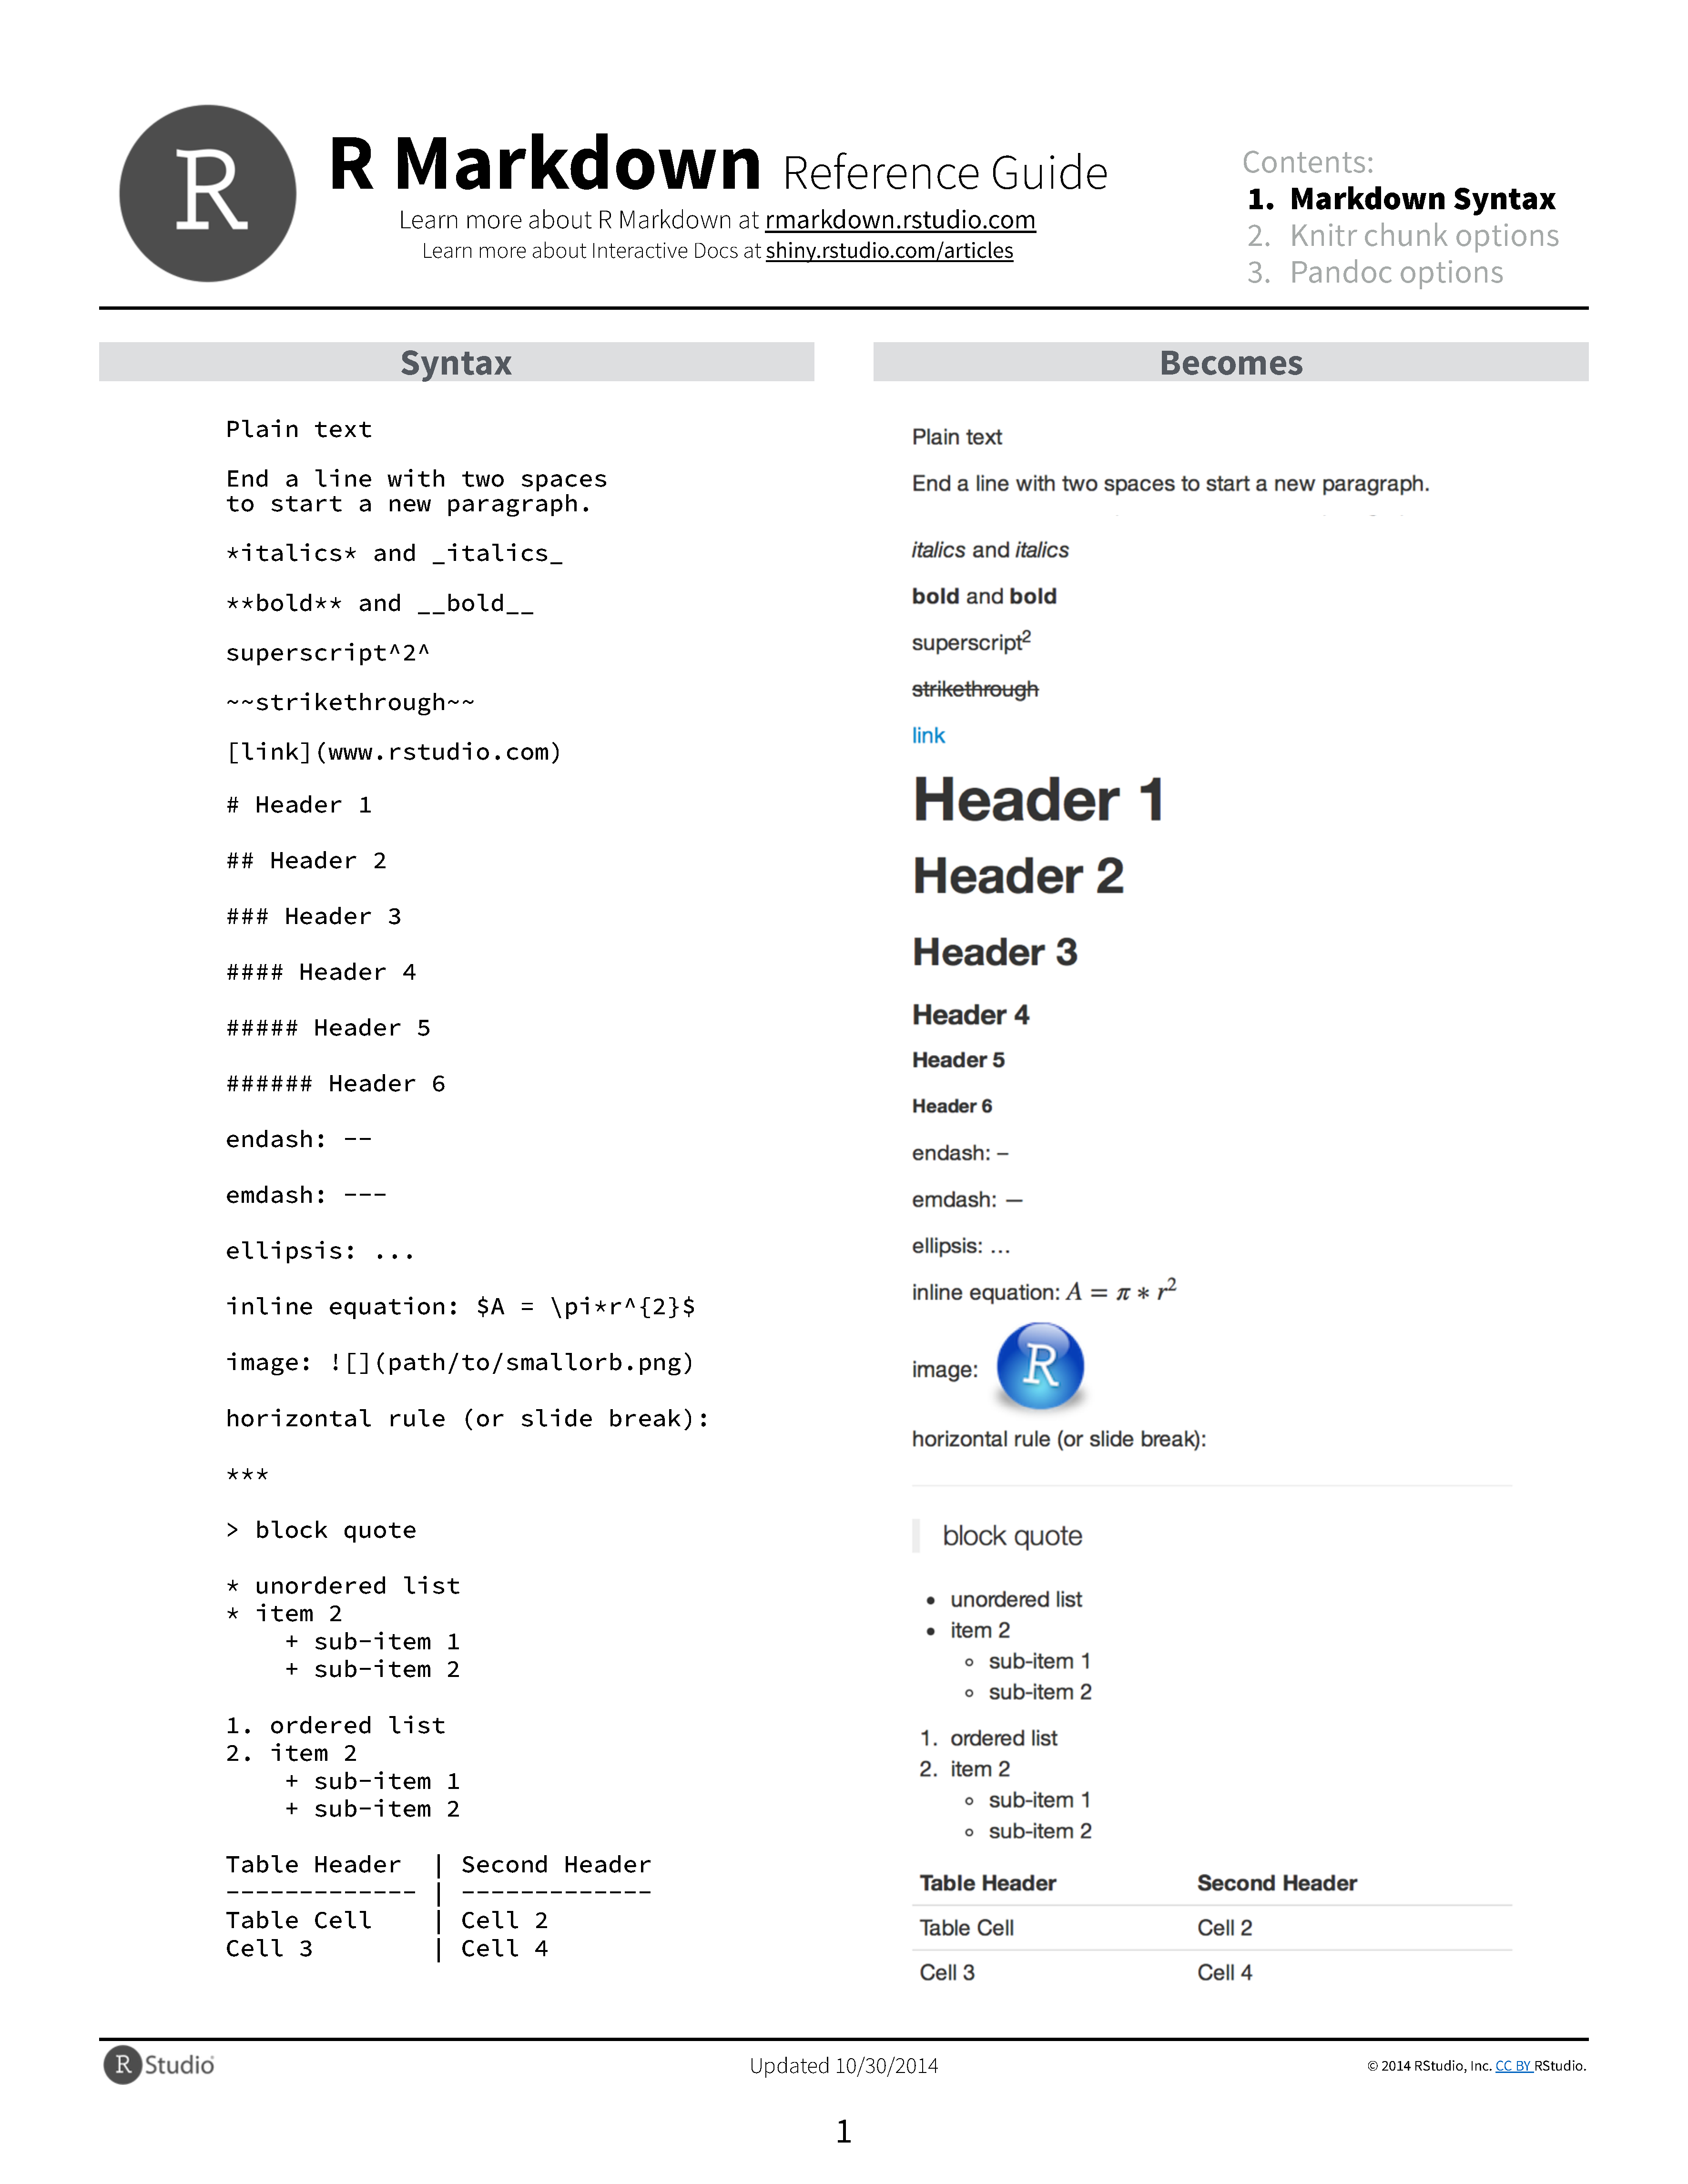
\includegraphics{imgs/rmarkdown-reference.pdf}
\end{frame}

\begin{frame}{Lógica, instalação e recursos adicionais}
\protect\hypertarget{luxf3gica-instalauxe7uxe3o-e-recursos-adicionais}{}
\begin{itemize}
\item
  Pandoc e knitr
\item
  LaTeX
\end{itemize}
\end{frame}

\begin{frame}{O básico}
\protect\hypertarget{o-buxe1sico}{}
Cabeçalho

-- opções e possibilidades

Escrita

Chunks

-- opções -- nomes

Formatos de saída
\end{frame}

\begin{frame}{Saídas}
\protect\hypertarget{sauxeddas}{}
Documentos estáticos

Documentos Interativos

Dashboards

Apresentações

Livros

Sites

Modelos
\end{frame}

\begin{frame}{}
\protect\hypertarget{section-3}{}
\href{https://rmarkdown.rstudio.com/}{Site do RMarkdown}

IMPORTANTE!

\href{https://rmarkdown.rstudio.com/gallery.html}{Galeria para
replicação}
\end{frame}

\begin{frame}{Documentos}
\protect\hypertarget{documentos}{}
\begin{itemize}
\item
  HTML documents for web publishing.
\item
  PDF documents for printing. Example Code
\item
  Microsoft Word documents for Office workflows.
\item
  Tufte styled documents for handouts.
\end{itemize}
\end{frame}

\begin{frame}{Documentos Interativos}
\protect\hypertarget{documentos-interativos}{}
\begin{itemize}
\item
  Combine R Markdown with htmlwidgets or the shiny package to make
  interactive documents.
\item
  Add interactive graphics with htmlwidgets, such as the leaflet map
  widget.
\item
  Embed htmlwidgets such as dygraphs and datatables directly into your
  reports.
\item
  Shiny components and htmlwidgets will work in any HTML based output,
  such as a file, slide show or dashboard.
\end{itemize}
\end{frame}

\begin{frame}{Dashboards}
\protect\hypertarget{dashboards}{}
\begin{itemize}
\item
  Use flexdashboard to create dashboards with gauges and value boxes.
\item
  Add interactive graphics to a dashboard with htmlwidgets.
\item
  Organize dashboards around a storyboard.
\end{itemize}
\end{frame}

\begin{frame}{Apresentações}
\protect\hypertarget{apresentauxe7uxf5es}{}
\begin{itemize}
\item
  Create pdf slides with Beamer.
\item
  Create HTML-based slides with Slidy.
\item
  Create HTML-slides with ioslides.
\item
  Create HTML-based slides with reveal.js.
\end{itemize}
\end{frame}

\begin{frame}{Livros}
\protect\hypertarget{livros}{}
\href{https://bookdown.org/yihui/rmarkdown-cookbook/}{O próprio
Cookbook}
\end{frame}

\begin{frame}{Sites}
\protect\hypertarget{sites}{}
R Markdown makes it easy to build webpages straight from .Rmd files.

\begin{itemize}
\item
  The R Markdown website is itself built with R Markdown. Example Code.
\item
  flexdashboard extends R Markdown to make administrative dashboards.
  Its website is also built from R Markdown. Example Code.
\item
  Bookdown extends R Markdown to make books. Its website is built with R
  Markdown and CSS styling. Example Code.
\item
  profvis provides profiling tools for R code, as well as a website made
  with R Markdown. Example Code.
\end{itemize}
\end{frame}

\begin{frame}{Modelos}
\protect\hypertarget{modelos}{}
\begin{itemize}
\item
  The JSS article template in the rticles package formats an R Markdown
  document to meet the style guidelines of the Journal of Statistical
  Software. Example Code
\item
  The rjournal article template in the rticles package formats an R
  Markdown document to meet the style guidelings of the R Journal.
  Example Code
\item
  The skeleton template is one of several provided in Bob Rudis'
  markdowntemplates package. Example Code
\item
  Steve Miller's CV template formats an R Markdown file into a
  Curriculum Vitae (CV). Example Code
\end{itemize}
\end{frame}

\hypertarget{live-coding}{%
\section{Live Coding}\label{live-coding}}

\begin{frame}{Paper em pdf}
\protect\hypertarget{paper-em-pdf}{}
RAP - Usando bibliografia

\href{http://www.codeplan.df.gov.br/wp-content/uploads/2020/06/Itapo\%C3\%A3.pdf}{PDAD}
\end{frame}

\begin{frame}{Relatório em html}
\protect\hypertarget{relatuxf3rio-em-html}{}
\href{http://www.codeplan.df.gov.br/wp-content/uploads/2018/02/Cartografia-das-compras-p\%C3\%BAblicas-de-bens-e-servi\%C3\%A7os-privados-no-DF.html}{Compras
públicas}

\href{https://rpubs.com/fredbsr/ANIPES}{ANIPES}
\end{frame}

\begin{frame}{Slides em html}
\protect\hypertarget{slides-em-html}{}
Usando CSS

\href{https://github.com/fredbsr/covid19br_OP}{Apresentação COVID}
\end{frame}

\end{document}
